\chapter{Secret Storage as a Service}
\label{chap:ssaas}

As discussed in Chapter~\ref{chap:challenges}, the reliance on third
parties inherent to many popular use cases poses a number of privacy
and security related challenges. Fortunately, cryptographic techniques
including encryption and authentication provide the necessary
primitives for building a systems that increases the security and
privacy of users by reducing their exposure to third party-related
abuses of trust. Such systems also provide additional security outside
of the traditional third-party risk model by ensuring that systems
such as mobile devices that are prone to loss or theft remain secure
even when outside the position of their owners. Unfortunately,
cryptography is not merely ``magic fairy dust'' that we can sprinkle
on any security or privacy problem to make it
disappear~\cite{smith2003}. Effectively using cryptographic technique
to secure our data involves ensuring that cryptography-employing
security and privacy enhancing solution are designed in a secure and
usable manner.

The crux to designing secure and usable cryptographic data security
solutions lies in providing secure and flexible secret storage systems
that can be leveraged to manage and store the cryptographic keys
associated with any such system. The failure of traditional
cryptographic systems to account for key management has led many such
systems to be unusable, insecure, and/or ill-adapted to modern use
cases. I propose the creation of a standardized Secret Storage as a
Service system designed to provide users with the necessary tools for
managing secrets such as cryptographic keys in a manner that allows
for a range of use cases and that avoids placing high degrees of trust
in any single third party. I present the design and justification of
such a system in this chapter.

\section{Architecture}
\label{chap:ssaas:arch}

Secret Storage as a Service (SSaaS) is a cloud architecture where
users utilize dedicated Secret Storage Providers (SSPs) in addition to
the traditional Feature Providers (FPs) like Amazon, Dropbox, Gmail,
or Facebook. An SSP is tasked with the storage of and access control
to a variety of user secrets from cryptographic keys to personal
data. In the normative case, users will limit themselves to storing
cryptographically-protect data on third-party FP servers while storing
the associated cryptographic keys protecting such data with a network
of SSPs. This allows SSPs to be selected on the basis of their
trustworthiness while traditional feature providers can be selected on
the basis of their feature sets. The SSaaS model differs from the
traditional cloud model by allowing users to distribute trust across
multiple third parties (or no third parties at all), ensuring that any
single entity need not be fully trusted, while still enabling many
popular use cases.

\subsection{Stored Secrets}

What kind of secrets do we store with an SSP? I believe that users
should be able to store arbitrary data with any SSP, allowing open
ended secret storage based applications. That said, the SSP model
works best when secrets stored are not inherently sensitive or
revealing when taken alone. This property helps to mitigate the amount
we must trust each SSP. Thus, storing secrets like cryptographic keys
that alone revel no private user data are generally preferable to
storing privacy revealing secrets like plain-text passwords, social
security numbers, etc. I do, however, leave the decision of what to
store with each SSP up to each user and application. I'll explore
various types of secret storage in Chapter~\ref{chap:apps}.

Another consideration related to what secrets to store with an SSP is
size. I anticipate SSP-based storage selling at a premium price vs
more traditional cloud storage options like Amazon
S3~\cite{amazon-s3}. This is due to the difference in priorities
between Secret Storage and generic cloud storage. An SSP is primarily
concerned with safeguarding user secrets and faithfully implementing a
user's access control specifications for each secret. These priorities
may very well incur additional costs not present in more traditional
cloud storage environments: e.g. the need to locate data centers in
specific legal jurisdictions, a greater emphasis of resistant to
compelled violations via legal representation, etc. Thus, it may be
desirable for the user to minimize the amount of data stored with an
SSP as a cost optimization: again making use cases such as storing
cryptographic keys with an SSP while storing the encrypted data with a
more traditional provider desirable.

For these reasons, I feel that storing cryptographic keys with an SSP
is a common enough use case that some SSPs may specifically optimize
for it. Such ``Key Storage as a Service'' (KSaaS) SSPs represent a
subset of the general SSaaS model.

\subsection{Secret Storage Providers}

In the SSaaS model, SSPs will offer a standard set of features. These
include a standardized interface, access control primitives, and
auditing capabilities. These features provide the basis of building
privacy-preserving SSaaS-backed applications.

\subsubsection{Secret Storage}

At its core, an SSP provider is offering a key:value data storage
model. Each secret is tagged with a key: a unique identifier,
potentially a UUID~\cite{leach2005} or similar unique ID standard. The
value associated with each key is then the user secret itself, be it a
cryptographic key, personal user data, or arbitrary secret
value. Users are able to query each SSP for the value associated with
a given ID, or to add new secrets to each SSP.

Optionally, SSPs may provide versioning of each id:secret pair. This
may be desirable for use cases where the user wishes to share data
with other users while maintaining the ability to revoke shared access
to future versions of a data set. Such ``lazy
revocation''~\cite{kallahalla2003} capabilities can be built atop
versioning schemes that maintain access control information on a
per-version basis.

I foresee each SSP exposing its key-value secret store via a RESTful
HTTPS-based API. The ubiquity of RESTful interfaces in modern
applications ensures that such an interface will allow simple
communication between a client and the SSP across a wide variety of
platforms. This interface will expose create, read, modify, delete
semantics similar to most existing key:value stores. In fact, I assume
that most SSP implementations will use an off-the-shelf key-value
store as the backend for storing user secrets. I intend for SSPs to
utilize a standard API in order to allow user to interact with
multiple SSPs and transfer their secrets between SSPs.

\subsubsection{Access Control}

The SSP data model associates an access control specification with
each id:secret pair (or in a versioned system, with each
id:version:secret set). This specification governs the manner in which
a given secret can be accessed. Such specification will be provided
and controlled by individual users for each secret they store with the
SSP. The SSP is in charge of faithfully enforcing the access control
specification.

An access control specification dictates who can create, access,
modify, or delete each secret. It contains information regarding both
authentication (how a user proves they are who they claim to be) as
well as authorization (what permissions each authenticated user is
granted). I foresee SSPs offering a standard access control framework
in order to promote interoperability between multiple SSPs.

It's important that the SSP access control model remain
flexible. Since an SSP may be asked to store a variety of secrets in
support of a range of use cases, the access control model must be
expressive enough to avoid artificially limiting the user to specific
use cases or secrets. For example, one use case might require a single
user to satisfy multiple challenges in order to gain access to a
highly sensitive secret while another might allow autonomous access
from system possessing an approved token during specific times of day
to access secrets used by autonomous processes (e.g. a data-center
server booting an encrypted hard disk or using a secure backup
system).

In addition to the key:value storage API operations discussed
previously, an SSP will also expose API endpoints for manipulating the
access control parameters associated with each secret as part if the
standard REST API. This interface will allow users to update access
control information to allow data sharing with other users, revoke
prior shared access, etc. This interface will, in turn, require it's
own access control specification to ensure that only approved
modifications can be made to any secret's access control rules.

\subsubsection{Auditing}

In addition to access control, each SSP should provide auditing
information related to the manner in which each id:secret pair is
accessed or modified. This information is useful to the user in order
to provide additional transparency into the manner in which secrets
are utilized. This auditing can be as simple as basic logging of all
secret access or as complex as a system that automatically analyzes
access patterns to try to detect anomalies that might indicate
potential trust violations.

Auditing information is useful to users for several reasons. In the
event that user data or secrets are ever unintentionally leaked or
compromised, audit information can provide a valuable indication of
the scope of the damage. Furthermore, auditing plays an important role
in allowing users to understand the semantics of access revocations:
since it's unfeasible to revoke access to data another user has
already read (and potentially copied out-of-band), audit information
provides a user with the scope of potentially revocable outstanding
authorization allowances. E.g. if User A shares a secret with User B
by granting them read access to it via their SSP, but then decides
they'd rather revoke that access, User A can check the audit logs to
determine if User B has yet accessed the shared secret and thus
whether or not guaranteed revocation is even possible.

As in the prior cases, an SSPs auditing capabilities will need to be
exposed via a REST interface to allow client applications to leverage
audit data. Likewise, audit API functions will need their own set of
access control specifications in order to control who has access to
audit information or the ability to delete that information. As
before, standardizing this interface is desirable from an SSP
interoperability standpoint.

It may also be desirable for SSPs to employ some form of
publicly-verifiable audit trail, similar to the concepts discussed in
\cite{blaze1996} or \cite{laurie2013}. Alternatively, such systems
might today be constructed using block-chain-based primitives such as
those available in the BitCoin crypto-currency
network~\cite{Nakamoto2008}. Such systems might provide more robust
variants on the ``warrant cannery'' concept that has recently become
popular amongst a range of third-party services providers as a counter
measure against secret warrants, subpoenas, and court
orders~\cite{eff-canary}. The semi-centralized nature of SSPs make
them a desirable point at which to audit and detect unauthorized
access requests for user data.

\subsection{Clients}

While SSPs form one half of the SSaaS architecture, the other half is
formed by clients connecting to and leveraging data from
SSPs. Chapter~\ref{chap:apps} discusses potential SSaaS use cases and
applications in detail. I outline some of the basics of SSaaS client
deign and operation here.

An SSaaS client is any system designed to connect to and utilize a
Secret Storage Provider service. Clients communicate with one or more
SSP via the SSaaS API. Clients can store and retrieve secrets with
each SSP, managing secret access control settings, and retrieve secret
access audit info. Examples of SSaaS client applications include
encrypted file systems, secure communication systems, dedicated
crypto-processing systems, etc. Any system that stands to benefit from
offloading secret storage and management to a dedicated system, either
for the purpose of gaining benefits from the logically centralized
nature of an SSP (e.g. for the purpose of accessing secrets from
multiple devices or for sharing them with multiple users) or simply to
avoid implementing a full secret management and access control stack
locally, is a good candidate for integration into an SSaaS
architecture.

Is the simplest case, each SSaaS client communicates with a single
upstream SSP via a standard SSaaS protocol. The standardized protocol
allows the end-user to specify which SSP they wish to use, and to
change SSPs as desired. The downside to such arrangements lies in the
fact that storing each secret with only a single SSP raises both trust
and availability concerns (the details of which are discussed
below). To overcome such concerns, I believe it will often be
desirable for each SSaaS client to interact with a network of several
upstream SSPs. In this situation, each secret can be sharded between
multiple SSPs - increasing reliability while also reducing trust.

Such multi-SSP arrangement, however, raise client side management
issues. How are access control rules shared between SSPs? How does the
client keep multiple SSPs in sync? And so on... Answering such
questions is some of the work I propose to undertake in
Chapter~\ref{chap:planned}. The complexity of such solutions will
likely call for the creation of a standardized SSaaS client library
that can be utilized by multiple applications. Such a library avoids
the need for each SSaaS client to reimplement SSaaS communication and
management primitives directly. Furthermore, it may also be desirable
to create a common SSaaS management application. Many of the
SSaaS-related management features, e.g. setting up access control
requirements, checking audit logs, etc, are common across all SSaaS
client applications. It may thus be desirable to offload such
functions to a general SSaaS client management applications in cases
where such functions need not be tightly coupled with a given
SSaaS-backed applications. Such offloading allows the primary
SSaaS-backed applications to focus purely on the secret storage and
retrieval side of the SSaaS API while dedicated management
applications handle the access control and auditing side of the SSaaS
API.

\section{Economics}
\label{chap:ssaas:economics}

Part of the the argument in favor of the SSaaS model is
economics. Today, users primarily select cloud services on the basis
of their features. When they pay for these services, they're primarily
paying to support the core features such service provide. Privacy and
security, while concerns, are often secondary goals. Furthermore, on
many free cloud services, the ability to harvest user data is the
basis of the service provider's business model. These situations
create a number of perverse incentives in terms of a traditional
feature provider's goals with respect to user security and
privacy~\cite{anderson2001}. In the first case, the feature provider
simply does not prioritize user security since that's not the primary
basis on which users are choosing to pay for a service. In the second
case, a feature provider might actively work to subvert user security
and privacy in order to further leverage user data to generate income.

The SSaaS model aims to rectify these issues by introducing SSP actors
whose primary goal is the protection of user secrets and from whom
users purchase secret storage services on the basis of security and
privacy guarantees first and foremost. Thus, SSaaS's ability to
separate secret storage duties from feature provider duties allows
users to purchase each service on the basis of its associated merits,
avoiding the issues associated with putting features in direct
competition with security and privacy: a competition that security and
privacy have historically lost. Given such separation, independent
markets can form around feature provision and secret protection, all
optimized for the respective priorities of each field.

Beyond the removal of perverse incentives brought about by the
separation of SSPs for FPs, it will also be desirable to encourage a
competitive market amongst multiple SSP providers. In order to achieve
such a market, I advocate for the standardization of a single
inter-compatible SSaaS protocol. Such a standard protocol gives users
a high degree of mobility between competing SSPs providers, avoiding
vendor lock-in. This mobility, in turn, increases the competitive
pressures between providers. In short, the aim of an SSaaS ecosystem
is to make security and privacy tradable commodities, and to leverage
market powers to price and improve both. A competitive market for
secret storage has a number of security and privacy enhancing
benefits:

\begin{packed_desc}
\item[Reputation:] If users can easily switch between SSPs, it forces
  SSPs to compete on the basis of their security and privacy
  preserving reputations. SSPs who can do a superior job avoiding the
  trust violations discussed in Chapter~\ref{chap:trust} can attract
  more users and/or command a higher price for their services. Since a
  SSP's reputation is tied solely to their ability to faithfully
  protect user secrets, they will not be able to ``iron over'' any
  privacy-related reputation failings with superior end-user feature
  sets -- as many traditional cloud providers do today\footnote{As an
    example, consider Facebook's numerous trust
    violations~\cite{goel2014, lomas2014, tsukayama2014} and the fact
    that such violations have had no noticeable impact on the number
    of people using Facebook~\cite{foster2014}. An SSP would enjoy no
    such network benefit from additional services beyond secret
    storage were they to violate user's trust; instead, users would
    simply switch to a new SSP.}.
\item[Multiple Providers:] A healthy ecosystem of competing SSPs will
  allow users to select from multiple independent providers over which
  they may shard a single secret. As I'll discuss below, this
  multi-SSP practice provides a number of benefits over relying on a
  single SSP, from additional trust reduction to redundancy.
\item[Cost:] As in other competitive markets, having a number of
  competing providers will allow the user to select a provider that
  offers the best combination of cost and service.
\end{packed_desc}

The SSaaS model also provides business benefits related to
insurance. Having a dedicated entity in charge of protecting user
secrets (and by proxy, any other data protected by those secrets)
simplifies the process of evaluating risk and liability related to the
protection of sensitive data. Similar to the model used by Certificate
Authorities, SSPs could provide insurance polices to their users to
indemnify them against any loss relating from a trust violation on the
part of the SSP. Likewise, SSPs would underwrite such user-facing
insurance polices with their own insurance polices provided by
independent third-party insurers. These insurers would need to perform
independent audits of SSP infrastructure and polices in order to
evaluate trust violation risk, further enticing SSPs to fundamentally
deign themselves for the avoidance of such trust violations. Such
insurance benefits are not as readily available in the mixed trust +
feature cloud ecosystem of today since it's far harder to evaluate the
privacy violation risk of a company whose primary objectives are more
complex then secret storage alone. The increasing regulation of user
privacy rights and the penalties associated with violating user
privacy further incentive a system where privacy and security are
severable properties that can be independently regulated, evaluated,
and indemnified -- unconnected to the user-facing feature set of a
given third-party service.

Likewise, SSaaS provides compliance benefits to users storing highly
regulated data. Instead of having to individually verify that each
end-user cloud service meets the requirements of a specific data
storage regulations, a user could instead simply make sure that their
SSP meets the necessary regulations. Once verified, a single SSP could
be reused with multiple FPs without having to undergo further
compliance verification. SSPs might even proactively obtain specific
compliance certifications to make it easy for their users to comply
with specific regulations, regardless of which feature-providing cloud
service a user wishes to leverage. Such practices would likely prove
highly beneficial in tightly-regulated fields such as health care
(e.g. requiring HIPPA~\cite{hippa} compliance), education
(e.g. requiring FERPA~\cite{ferpa} compliance), and online payment
processing (e.g. requiring PCI DSS~\cite{pcidss} compliance).

\section{Security and Trust}
\label{chap:ssaas:trust}

As mentioned in Chapter~\ref{chap:trust}, use cases that involve
splitting user data into cryptographically-protected core data and the
associated cryptographic keys (e.g. secrets) and storing each with
separate providers inherently decrees the amount that any single
provider must be afforded. If, however, we wish to store unencrypted
user data directly with an SSP, potentially because a given use case
can't easily be split into encrypted data and encryption keys, we must
place a higher degree of trust in an SSP. In the split encrypted data
+ cryptographic secrets use case, we must only trust the SSP with the
storage (\emph{S}) and metadata (\emph{M}) capabilities, the same
capabilities with which we must trust the FP. But in the case where an
SSP directly stores raw user data, we must expand their capability
profile to also include the access (\emph{R} ) and manipulation
(\emph{W}) capabilities. Are SSPs any more worthy (i.e. less likely to
violate) this increased level of trust than a traditional FP?

Even in such a worst-case trust scenario, I believe that SSPs are less
likely to violate user trust. As outlined in
\S~\ref{chap:ssaas:economics}, SSPs have economic incentives well
aligned with upholding a user's trust where as traditional FPs often
have economic incentives in direct conflict with upholding user
trust. This fact alone decreases their likelihood of trust violation
by disincentivizing implicit violations (\emph{P}-type) and putting a
higher premium on avoiding unintentional (\emph{U}-type), insider
(\emph{I}-type), and outsider (\emph{O}-type) violations. I thus feel
that users are thus better off trusting SSPs with raw sensitive data
than FPs.

\begin{figure}[t]
  \centering
  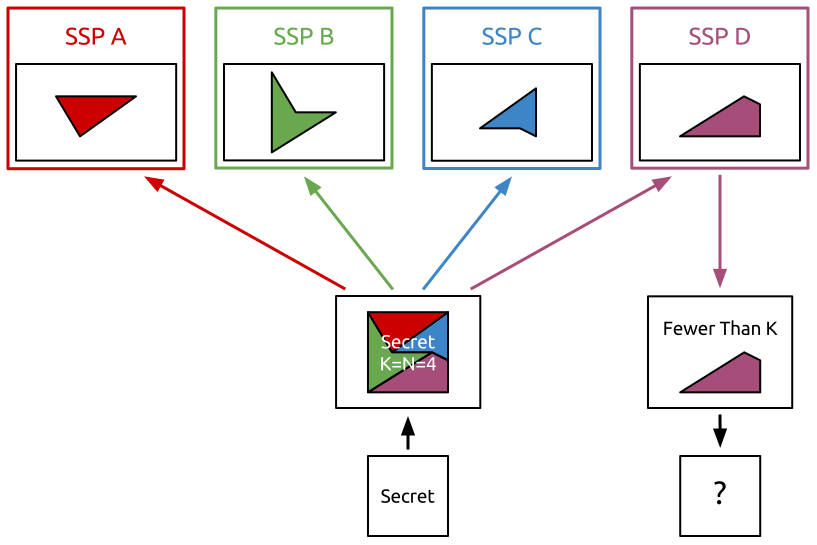
\includegraphics[height=200px]{./figs/out/Arch-Sharded.pdf}
  \caption{Sharding Secrets Between Multiple Providers}
  \label{fig:ssaas-sharded}
\end{figure}

None the less, it's best if users can avoid placing high degrees of
trust in any third party, FP or SSP. Fortunately, there is a viable
alternative for avoiding additional trust even in the raw-secret
storage SSP use case (and for further reducing trust even in the split
use case): cryptographically sharding a single user secret across
multiple SSPs. As shown in Figure~\ref{fig:ssaas-sharded}
Cryptographic secret sharing systems such as Shamir's $(k, n)$
threshold scheme~\cite{shamir1979} ensure that a secret split into $n$
shares can not be reassembled using fewer than $k$ shares in an
information theoretically secure manner\footnote{Information-theoretic
  security is an even higher level of security guarantee then
  traditional cryptographic security. Where as cryptographic security
  relies on assumptions about what kinds of math problems are or are
  not hard for computers to solve, information-theoretic security
  requires no such assumptions -- instead deriving security from
  fundamental and universal properties of information theory.}. Such
schemes could easily be applied in an SSaaS ecosystem to avoid
affording (\emph{R}) and (\emph{W}) capabilities to an SSP, even when
storing raw user data. In addition, secret sharing schemes have
benefits related to redundancy and data availability. Since $(k, n)$
threshold schemes include redundant shares in any case where $n > k$,
users can split their secrets into $n$ shards and insure that their
secrets will be recoverable as long as at least $k$ SSPs remain
operational and in possession of the stored shard. As such I foresee
sharding secrets, be they cryptographic keys or raw data, across
multiple SSPs being a standard best-practice in SSaaS ecosystems for
both the trust reduction and increased reliability benefits such
practice incur.

Even with secret sharing, as in the key-storage use case, users are
still at risk of a successful trust violation should multiple SSPs
collude to betray their secrets (\emph{L}-type violation) or should
multiple SSPs be compelled to turn over user data to a single entity
(\emph{C}-type violation). As such, we are interested in selecting a
set of SSPs across which to shard our secrets that minimize \emph{L}
and \emph{C}-type violation risk. Thus, in addition to the
reputation-based selection criteria outlined in
\S~\ref{chap:ssaas:economics}, I propose introduce several additional
SSP selection criteria:

\begin{packed_desc}
\item[Geopolitical Diversity] An ideal set of SSPs would be located
  across a range of non-cooperating geopolitical domains. This will
  greatly decrease the likelihood of a (\emph{C}-type violation) by
  ensuring that no single entity has the ability to compel multiple
  SSPs to surrender user data.
\item[Ownership Diversity] Similarly, a user should only select SSPs
  owned and operated by independent entities. This decreases the
  likelihood of an (\emph{L}-type violation) by ensuring no single
  entity can instruct multiple SSPs to collude.
\end{packed_desc}

If the user selects a diverse set of SSPs, all with strong
privacy-preserving reputations, I believe that they have a reasonable
likelihood of avoiding a successfully series of trust violations
resulting in the compromise of user privacy or security.

%%  LocalWords:  SSaaS SSPs FPs SSP HTTPS TBD SSaaS's SSP's FP HIPPA
%%  LocalWords:  Shamir's BitCoin FERPA PCI DSS
